\documentclass[11pt]{beamer}
\usepackage[utf8]{inputenc}
\usepackage{graphicx, epsfig}
\usepackage{amsmath,mathrsfs,amsfonts,amssymb}
%\usepackage{subfig}
\usepackage{floatflt}
\usepackage{epic,ecltree}
\usepackage{mathtext}
\usepackage{fancybox}
\usepackage{fancyhdr}
\usepackage{multirow}
\usepackage{enumerate}
\usepackage{epstopdf}
\usepackage{multicol}
\usepackage{algorithm}
\usepackage[noend]{algorithmic}
\usepackage{tikz}
\usepackage{blindtext}
\usetheme{default}%{default}%{Singapore}%{Warsaw}%{Warsaw}%{Darmstadt}
\usecolortheme{default}
\setbeamerfont{title}{size=\Huge}
\setbeamertemplate{footline}[page number]{}


\makeatletter
\newcommand\HUGE{\@setfontsize\Huge{35}{40}}
\makeatother    

\setbeamerfont{title}{size=\HUGE}
\beamertemplatenavigationsymbolsempty

% latin bold lower
\newcommand{\ba}{\mathbf{a}} 
\newcommand{\bc}{\mathbf{c}} 
\newcommand{\be}{\mathbf{e}} 
\newcommand{\bh}{\mathbf{h}} 
\newcommand{\bp}{\mathbf{p}} 
\newcommand{\bt}{\mathbf{t}} 
\newcommand{\bs}{\mathbf{s}} 
\newcommand{\bu}{\mathbf{u}} 
\newcommand{\bv}{\mathbf{v}} 
\newcommand{\bw}{\mathbf{w}} 
\newcommand{\bx}{\mathbf{x}} 
\newcommand{\by}{\mathbf{y}} 
\newcommand{\bz}{\mathbf{z}} 

% latin bold upper
\newcommand{\bA}{\mathbf{A}} 
\newcommand{\bB}{\mathbf{B}} 
\newcommand{\bC}{\mathbf{C}} 
\newcommand{\bI}{\mathbf{I}} 
\newcommand{\bL}{\mathbf{L}} 
\newcommand{\bM}{\mathbf{M}} 
\newcommand{\bQ}{\mathbf{Q}} 
\newcommand{\bT}{\mathbf{T}} 
\newcommand{\bU}{\mathbf{U}} 
\newcommand{\bV}{\mathbf{V}} 
\newcommand{\bW}{\mathbf{W}} 
\newcommand{\bX}{\mathbf{X}} 
\newcommand{\bY}{\mathbf{Y}} 
\newcommand{\bZ}{\mathbf{Z}} 

% latin cal upper
\newcommand{\cG}{\mathcal{G}} 
\newcommand{\cL}{\mathcal{L}} 
\newcommand{\cN}{\mathcal{N}} 
\newcommand{\cS}{\mathcal{S}} 
\newcommand{\cT}{\mathcal{T}} 
\newcommand{\cW}{\mathcal{W}} 
\newcommand{\cX}{\mathcal{X}} 
\newcommand{\cZ}{\mathcal{Z}} 

% latin bb upper
\newcommand{\bbE}{\mathbb{E}} 
\newcommand{\bbI}{\mathbb{I}} 
\newcommand{\bbP}{\mathbb{P}} 
\newcommand{\bbR}{\mathbb{R}} 

% greek bold lower
\newcommand{\bepsilon}{\boldsymbol{\epsilon}} 
\newcommand{\btheta}{\boldsymbol{\theta}} 
\newcommand{\blambda}{\boldsymbol{\lambda}} 
\newcommand{\bpi}{\boldsymbol{\pi}} 
\newcommand{\bmu}{\boldsymbol{\mu}} 
\newcommand{\bsigma}{\boldsymbol{\sigma}} 
\newcommand{\bphi}{\boldsymbol{\phi}} 

% greek bold upper
\newcommand{\bSigma}{\boldsymbol{\Sigma}} 

\DeclareMathOperator*{\argmin}{arg\,min}
\DeclareMathOperator*{\argmax}{arg\,max}
\newcommand{\createdgmtitle}[1]{\title[\hbox to 56mm{Mathematical Forecasting Methods \hfill\insertframenumber\,/\,\inserttotalframenumber}]
	{\vspace{1.5\cm} \\ Mathematical Forecasting Methods \\ {\Huge Лекция #1}}
	\author{}
	\institute{
	МФТИ
	} 
	\date{Осень, 2023}
}

\newcommand\myfootnote[1]{%
  \tikz[remember picture,overlay]
  \draw (current page.south west) +(1in + \oddsidemargin,0.5em)
  node[anchor=south west,inner sep=0pt]{\parbox{\textwidth}{%
      \rlap{\rule{10em}{0.4pt}}\raggedright\scriptsize \textit{#1}}};}

\newcommand\myfootnotewithlink[2]{%
  \tikz[remember picture,overlay]
  \draw (current page.south west) +(1in + \oddsidemargin,0.5em)
  node[anchor=south west,inner sep=0pt]{\parbox{\textwidth}{%
      \rlap{\rule{10em}{0.4pt}}\raggedright\scriptsize\href{#1}{\textit{#2}}}};}
\createdgmtitle{12}
\usepackage{tikz}
\usepackage{amsmath}
\usepackage[english,russian]{babel}
\usepackage[labelformat=empty]{caption}

\usepackage{graphicx,animate}
\usepackage{animate}
\usepackage{svg}
\usepackage{subcaption}

\usepackage{ stmaryrd }

\usetikzlibrary{arrows,shapes,positioning,shadows,trees}
\newcommand*{\defeq}{\stackrel{\text{def}}{=}}
\newcommand{\tensor}[1]{\underline{\textbf{#1}}}
\newcommand{\M}[1]{\textbf{#1}}
\newcommand{\norm}[1]{\lVert #1 \rVert }
%--------------------------------------------------------------------------------
\begin{document}
%--------------------------------------------------------------------------------
\begin{frame}[plain]
%\thispagestyle{empty}
\titlepage
\end{frame}
%=======
\begin{frame}{Напоминание}
 

\begin{itemize}
    \item Два способа представить каноническое разложение:
$$\tensor{X} = \sum_{r=1}^R \M{b}_r^{(1)} \circ \M{b}_r^{(2)} \circ ... \circ \M{b}_r^{(N)} =  \llbracket \tensor{I}; \M{B}^{(1)}, \M{B}^{(2)}, \dots,  \M{B}^{(N)} \rrbracket$$

    \item Алгоритм ALS позволяет приближенно находить каноническое разложение тензора.

    \item Норма Фробениуса
    $$\lVert\tensor{A}\rVert_F = \sqrt{\sum_{i_1,...,i_N}a_{i_1,...,i_N}^2} = \lVert vec(\tensor{A}) \rVert_2$$
    \item (дополнение) Норма Фробениуса для тензоров порождается скалярным произведением (тензоры $\tensor{A}$ и $\tensor{B}$ имеют одинаковый порядок и их размерности совпадают):
    $$ \langle \tensor{A}, \tensor{B} \rangle = \sqrt{\sum_{i_1,...,i_N}a_{i_1,...,i_N}b_{i_1,...,i_N}} $$
\end{itemize}

\end{frame}
%=======
\begin{frame}{Разложение Такера}
$\tensor{X} \in \mathbb{R}^{I_1 \times I_2 \times \dots \times I_N}$ - тензор $N$-ого порядка.

\begin{itemize}

    \item Каноническое разложение может быть представлено в виде произведения Такера с единичным тензором $\tensor{I}$ (или диагональным тензором $\underline{\Lambda}$) и набором фактор-матриц $\M{B}^{(1)}, \dots,  \M{B}^{(N)}$:
    $$\tensor{X} = \llbracket \tensor{I}; \M{B}^{(1)}, \dots,  \M{B}^{(N)} \rrbracket \quad \text{или} \quad \tensor{X} = \llbracket \underline{\Lambda}; \M{B}^{(1)}, \dots,  \M{B}^{(N)} \rrbracket$$
    
    \item Каноническое разложение - частный случай \textit{Разложения Такера}. Разложение Такера представляется в виде произведения Такера \textbf{произвольного} тензора $\tensor{G} \in \mathbb{R}^{R_1 \times  \dots \times R_N}$ (core tensor, \textit{центральный} тензор) и фактор-матриц $\M{U}^{(n)}$:
    $$ \tensor{X} = \big[ \tensor{G}; \M{U}^{(1)}, \dots, \M{U}^{(N)} \big] := \tensor{G} \times_1 \M{U}^{(1)} \times_2 \M{U}^{(2)} \times_3 \dots \times_N \M{U}^{(N)} $$
    \item Мультилинейный ранг тензора - вектор рангов его развёрток:
    $$\text{rank}_\text{ML}(\tensor{X}) = \Big(rank(\M{X}_{(1)}),...,rank(\M{X}_{(N)})\Big)$$
\end{itemize}
\end{frame}
%=======
\begin{frame}{Сингулярное Разложение (Singular Value Decomp., SVD)}
Для аналогии вспомним разложение в случае матриц.\\
Любая матрица $\M{X} \in \mathbb{R}^{m \times n}$ представима в виде

$$ \M{X}
    = \M{U} \Sigma \M{V}^{\intercal}
    = \Sigma \times_1 \M{U} \times_2 \M{V}
    = \llbracket \Sigma; \M{U}, \M{V}\rrbracket
$$
Здесь:
\begin{itemize}
    \item Матрицы $\M{U} \in \mathbb{R}^{m \times m}$, $\M{V} \in \mathbb{R}^{n \times n}$ - ортогональные матрицы
    \item $ \Sigma = \text{diag}(\sigma_1,...,\sigma_{min(m,n)}) \in  \mathbb{R}^{m \times n}$ --- диагональная матрица сингулярных чисел,
    где $\sigma_1\geq ... \geq \sigma_{\min (m,n)}\geq 0$
\end{itemize}
\begin{figure}
    \centering
    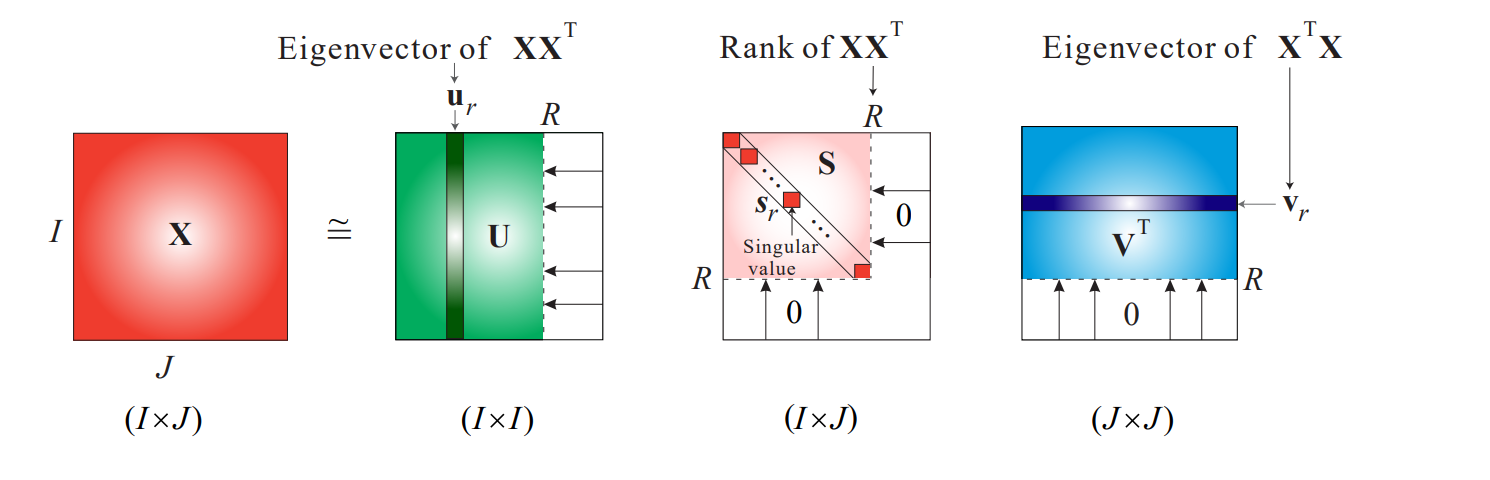
\includegraphics[width=0.9\textwidth]{lecture_12/figs/SVD.png}
\end{figure}
\end{frame}

%=======
\begin{frame}{Higher-order singular values decomposition}
В случае тензоров можно применить ту же логику, как и в матричном SVD.\\
Любой тензор $\tensor{X} \in \mathbb{R}^{I_1 \times ...\times I_N}$ представляется в виде 
$$ \tensor{X}
= \llbracket \tensor{S}; \M{U}^{(1)}, ... ,\M{U}^{(d)}\rrbracket
$$
При этом:
\begin{itemize}
    \item $\M{U}^{(k)} \in \mathbb{R}^{n_k \times n_k}$ - ортогональные матрицы (factor matrices), условие аналогичное матричному SVD.
    \item В тензоре $\tensor{S}$  подтензоры $\tensor{S}_{:,...,:,i_n,:,...,:}$ имеют свойства:
    \begin{itemize}
        \item $\langle \tensor{S}_{:,...,:,i_n,:,...,:}\tensor{S}_{:,...,:,j_n,:,...,:}\rangle_F = 0$ для $i_n\neq j_n$, где $i_n,j_n \in \overline{1, I_n}$, то есть подтензоры, соответствующие разным индексам вдоль одной моды, взаимно ортогональны,
        \item $\lVert \tensor{S}_{:,...,:,i_n,:,...,:} \rVert_F \geq \lVert \tensor{S}_{:,...,:,j_n,:,...,:} \rVert_F \text{  при  } i_n \geq j_n$, где норма $\sigma_{i_n} :=  \lVert \tensor{S}_{:,...,:,i_n,:,...,:} \rVert_F$ -- это сингулярное число развёртки вдоль соответствующей моды $\tensor{S}_{(n)}$.
    \end{itemize}
\end{itemize}

\end{frame}
% %=======
% \begin{frame}{Higher-order singular values decomposition}

% \begin{figure}
%     \centering
%     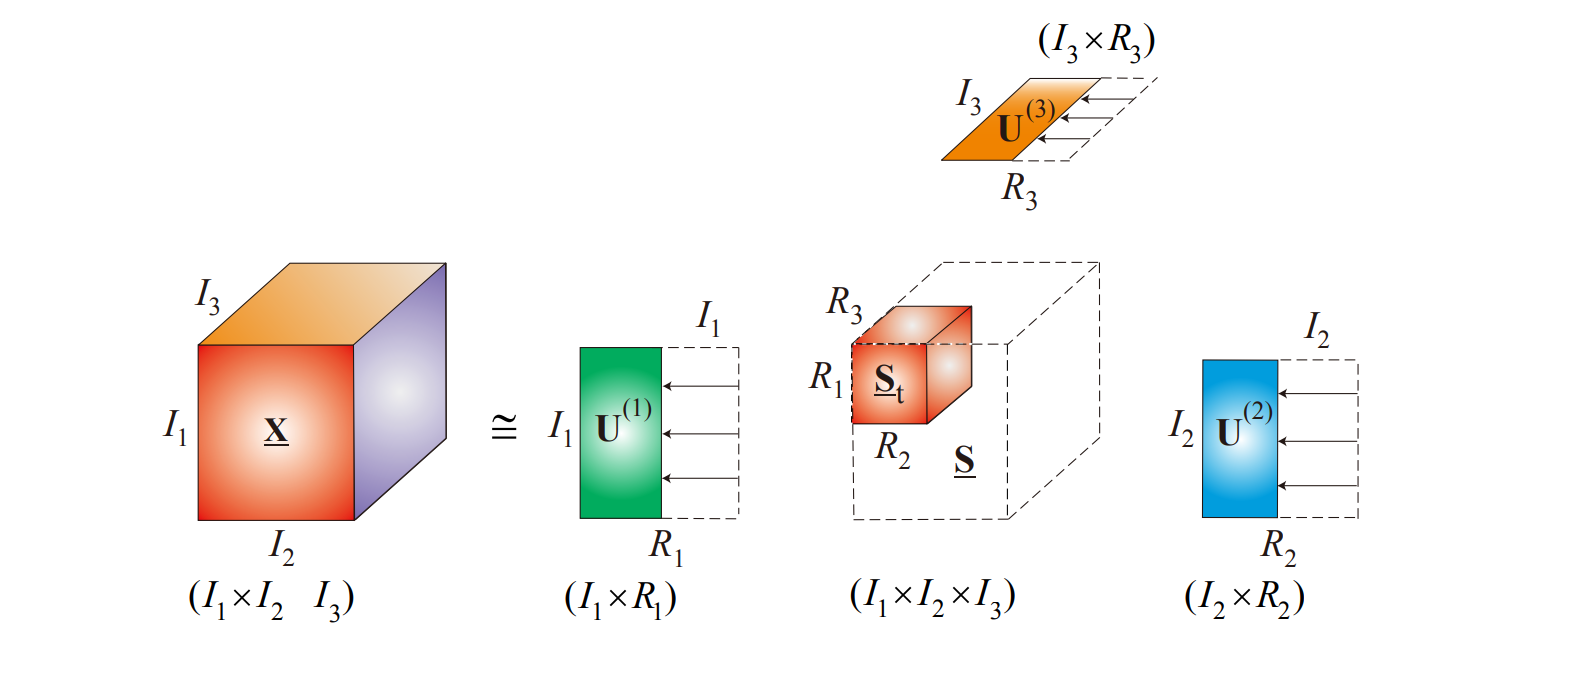
\includegraphics[width=0.9\textwidth]{lecture_12/figs/HOSVD.png}
% \end{figure}

% \end{frame}
% %=======
% \begin{frame}{Приближение тензора тензором меньшего ранга}

% $\lVert \tensor{A} - \tensor{T} \rVert_F \rightarrow \min_{\text{mlrank}(\tensor{T})<} $

% Сформулируем оптимизационную задачу как оптимизационную задачу на некотором линейном подпространстве


% \end{frame}

%=======
\begin{frame}{Алгоритм Sequentially Truncated Higher Order SVD}

\textbf{Input:} тензор $\tensor{X} \in \mathbb{R}^{I_1 \times \dots \times I_N}$ $N$-ого порядка и точность аппрксимации $\varepsilon$. \\
\textbf{Output:} HOSVD-разложение тензора  $\hat{\tensor{X}} = \llbracket \tensor{S}; \M{U}^{(1)}, \dots, \M{U}^{(N)} \rrbracket$, при этом $\norm{\tensor{X} - \hat{\tensor{X}}}_F \leq \varepsilon$.

\begin{enumerate}
    \item \textbf{for} $n = 1, \dots, N$ \textbf{do}:
    \item $\quad$ $\M{U}^{(n)}, \M{S}^{(n)}, \M{V}^{(n)} = \text{truncated\_SVD} \big(\M{X}_{(n)}, \frac{\varepsilon}{\sqrt{N}}\big)$ \\
    $\quad$ $\M{U}^{(n)} \in \mathbb{R}^{I_n \times R_n}, \M{S}^{(n)} \in \mathbb{R}^{R_n \times R_n}, \M{V}^{(n)} \in \mathbb{R}^{R_n \times I_1 \dots I_{n-1}I_{n+1} \dots I_N}$
    \item \textbf{end for}
    \item $\tensor{S} = \llbracket \tensor{X} ; \M{U}^{(1)}^\intercal, \dots,  \M{U}^{(N)}^\intercal \rrbracket$
    \item \textbf{return} тензор $\tensor{S}$ и фактор-матрицы $\M{U}^{(n)} \in \mathbb{R}^{I_n \times R_n}$
\end{enumerate}

\vspace{0.5cm}

\begin{itemize}
    \item Алгоритм \textbf{не даёт} наилучшего приближения в семействе тензоров соответствующего мультилинейного ранга (в отличие от SVD в случае матриц).
    \item Однако, для результирующего тензора $\hat{\tensor{X}}$ гарантируется свойство квазиоптимальности.
\end{itemize}


\end{frame}

%=======
\begin{frame}{Проблема Sequentially Truncated Higher Order SVD}
\begin{itemize}
    \item В отличие от стандартного SVD для матриц, Truncated Higher Order SVD не дает наилучшего мультилинейного рангового приближения, но удовлетворяет свойству квазинаилучшего приближения
$$
\norm{ \tensor{X} - \llbracket \tensor{S};\M{U}^{(1)},...,\M{U}^{(N)} \rrbracket} \leq \sqrt{N}\norm{\tensor{X} - \tensor{X}_{\text{Best}}}
$$,

где $\tensor{X}_{\text{Best}}$ --- это наилучшее приближение заданного мультилинейного ранга тензора $\tensor{X}$ для  нормы $\norm{\cdot}$.

\item Для поиска наилучшего приближения применяется аналог алгоритма ALS, называемый Higher Order Orthogonal Iteration (HOOI), который позволяет улучшить оценку фактор-матриц и центрального тензора в HOSVD.

\end{itemize}

\end{frame}

%=======

\begin{frame}{Алгоритм Higher Order Orthogonal Iteration}

\textbf{Input:} тензор $\tensor{X} \in \mathbb{R}^{I_1 \times \dots \times I_N}$ $N$-ого порядка.  \\
\textbf{Output:} Наилучшее приближение исходного тензора в виде разложения Такера c ортогональными фактор-матрицами $\M{U}^{(n)}$.

\begin{enumerate}
    \item Инициализируем разложение Такера $\tensor{X} = \llbracket \tensor{S}; \M{U}^{(1)}, \dots, \M{U}^{(N)} \rrbracket$ с помощью HOSVD.
    \item \textbf{repeat}
    \item $\quad$ \textbf{for} $n = 1, \dots, N$ \textbf{do}:
    \item $\quad$ $\quad$ $\tensor{Z} = \llbracket \tensor{X}; \M{U}^{(1)}^\intercal, \dots, \M{U}^{(n-1)}^\intercal, \M{I}, \M{U}^{(n+1)}^\intercal, \dots \M{U}^{(N)}\intercal \rrbracket$
    \item $\quad$ $\quad$ $\M{C} = \M{Z}_{(n)} \M{Z}^\intercal_{(n)} \in \mathbb{R}^{I_n \times I_n}$
    \item $\quad$ $\quad$ $\M{U}_{(n)}$ -- матрица из $R_n$ старших собств. векторов $\M{C}$
    \item $\quad$ \textbf{end for}
    \item $\quad$ $\tensor{G} = \llbracket \tensor{X} ; \M{U}^{(1)}^\intercal, \dots,  \M{U}^{(N)}^\intercal \rrbracket = \tensor{Z} \times_N \M{U}^{(N)}$
    \item \textbf{until} разность норм $\norm{\tensor{X}}_F - \norm{\tensor{G}}_F$ не перестанет убывать
    
    \item \textbf{return} тензор $\tensor{G}$ и фактор-матрицы $\M{U}^{(n)} \in \mathbb{R}^{I_n \times R_n}$
\end{enumerate}

\end{frame}

%=======
\begin{frame}{Разложение Такера}
\begin{figure}
    \centering
    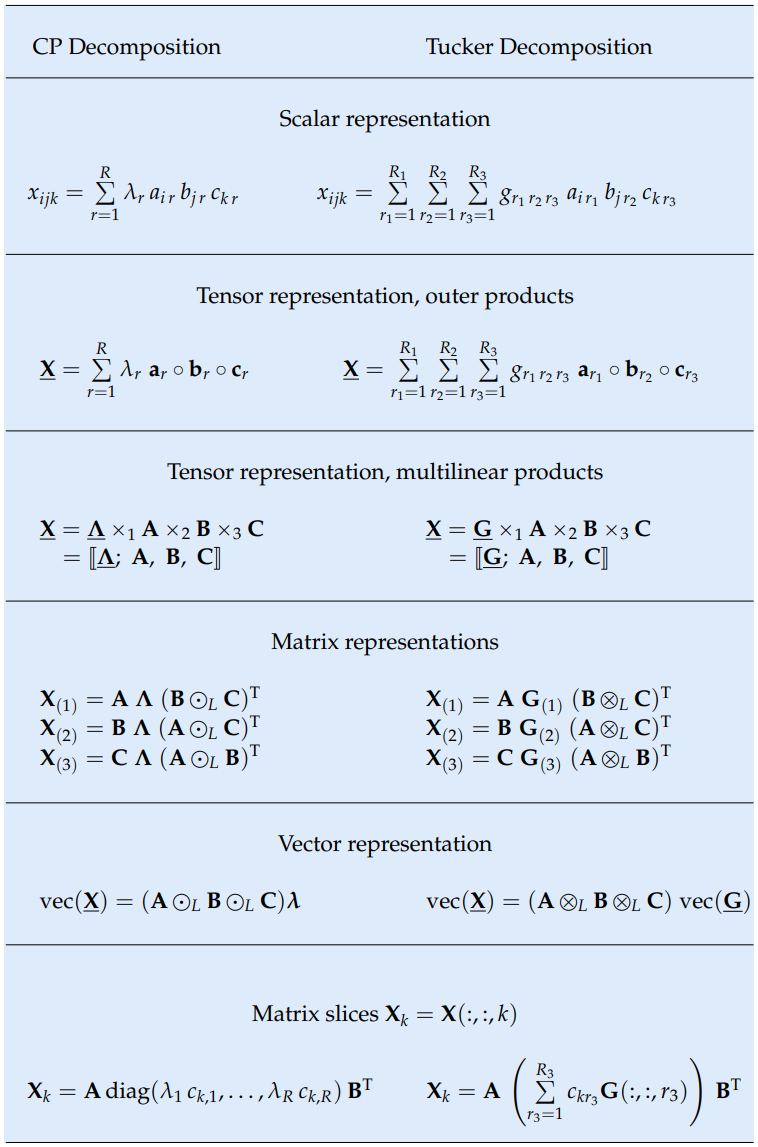
\includegraphics[width=0.5\textwidth]{lecture_12/figs/CP_Tuker.png}
\end{figure}
\end{frame}

%=======
\begin{frame}{Резюме}
\begin{itemize}
    \item Каноническое разложение в виде произведения Такера - частный случай разложения Такера.
    \item Используя разложение Такера, можно обобщить матричный SVD на тензорный случай HOSVD.
    \item HOSVD в чистом виде позволяет построить квазиоптимальное приближение исходного тензора, используя в своей основе матричный SVD.
    \item Один из алгоритмов позволяющих уточнить приближение тензора, HOOI,  позволяет итеративно находить матрицы факторов с помощью рассмотрения развёрток тензоров.
\end{itemize}
\end{frame}
\end{document} 